\documentclass[a4paper, 11pt]{article}
\usepackage[polish]{babel}
\usepackage[MeX]{polski}
\usepackage[utf8]{inputenc}
\usepackage[T1]{fontenc}
%\usepackage{times}
\usepackage{graphicx,wrapfig}
%\usepackage{anysize}
%\usepackage{tikz}
%\usetikzlibrary{calc,through,backgrounds,positioning}
\usepackage{anysize}
\usepackage{float}
%\usepackage{stmaryrd}
%\usepackage{amssymb}
%\usepackage{amsthm}
%\marginsize{3cm}{3cm}{3cm}{3cm}
%\usepackage{amsmath}
%\usepackage{color}
%\usepackage{listings}
%\usepackage{enumerate}
%\lstloadlanguages{Ada,C++}

\usepackage{listings} %do impotu kodu
\author{Marcin Jędrzejczyk  }
\title{Projekt AADL Automatu z przekąskami }


\newcommand{\HRule}{\rule{\linewidth}{0.5mm}} % Defines a new command for the horizontal lines, change thickness here
\newtheorem{defi}{Definicja}
\renewcommand{\contentsname}{Spis treści}
\renewcommand{\refname}{Bibliografia}
\renewcommand{\figurename}{Rysunek}


\begin{document}

%\maketitle	%robi stronê tytu³ow±
\begin{titlepage}


\center % Center everything on the page
%----------------------------------------------------------------------------------------
%	HEADING SECTIONS
%----------------------------------------------------------------------------------------

\textsc{\LARGE Akademia Górniczo-Hutnicza    \\im. Stanisława Staszica w Krakowie}\\[1.5cm] % Name of your university/college
\textsc{\Large Analiza i modelowanie oprogramowania}\\[0.5cm] % Major heading such as course name
%\textsc{\large Minor Heading}\\[0.5cm] % Minor heading such as course title

%----------------------------------------------------------------------------------------
%	TITLE SECTION
%----------------------------------------------------------------------------------------

\HRule \\[0.4cm]
{ \huge \bfseries Projekt AADL Automatu z przekąskami}\\[0.4cm] % Title of your document
\HRule \\[5.5cm]
 
%----------------------------------------------------------------------------------------
%	AUTHOR SECTION
%----------------------------------------------------------------------------------------

\begin{minipage}{0.4\textwidth}
\begin{flushleft} \large 
\emph{Autorzy:}\\
Marcin \textsc{Jędrzejczyk} \\


\end{flushleft}
\end{minipage}
~
\begin{minipage}{0.4\textwidth}
\begin{flushright} \large
\emph{Prowadzący:}\\
 Dr inż. Wojciech \textsc{Szmuc} % Supervisor's Name
\end{flushright}
\end{minipage} \\[5cm]

{\large \today}\\[3cm]
\vfill
\end{titlepage}
%----------------------------------------------------------------------------------------
%	DOCUMENT SECTION
%----------------------------------------------------------------------------------------
%\tableofcontents %robi spis tre¶ci	- 3 kompilacje
\newpage
\section{Automat z przekąskami }

\subsection{Wstęp}
 Automat sprzedający (automat vendingowy, ang. vending machine) – urządzenie służące do sprzedaży samoobsługowej. Można wyróżnić automaty sprzedające towary i usługi.\\
Projekt ten rozszerza poprzedni projekt pt.\"Projekt UML Automatu z przekąskami\" o perspektywę AADL.\\

\subsection{Założenia}
Założenia oraz wymagania nie zmieniły się w porównaniu do poprzedniego projektu.\\
Dla przypomnienia:
\begin{itemize}
\item Wybór produktu,
\item Uzyskanie informacji o cenie produktu,
\item Możliwość zrezygnowania z transakcji,
\item Zliczanie sumy wrzuconych pieniędzy,
\item Możliwość uzupełniania zasobami,
\item Wydanie zakupionego towaru,
\item Wydanie reszty,
\item Wyświetlenie powiadomień,
\end{itemize}

Należało jednak spojrzeć na nie ze strony niskopoziomowej.Przykładowo, jaka jest droga po urządzeniach i portach od przycisku do wypadnięcia danego produktu. A także jak będzie wyglądał kod w C.\\

Urządzenia, które wydzieliłem z automatu:
\begin{itemize}
\item Fotokomórka- sprawdza, czy produkt wypadł z automatu,
\item Liczydło- urządzenie do zliczania oraz sprawdzania autentyczności wpłacanej gotówki,
\item Podajnik- urządzenie, które upuszcza produkt do wnęki,
\item Przyciski- panel przycisków, na nim klient wystukuje kod produktu albo anuluje zakup,
\item Wyświetlacz- urządzenie do wyświetlania komunikatów.
\end{itemize}
 


\section{Diagramy AADL}


\begin{figure}[H]
\centerline{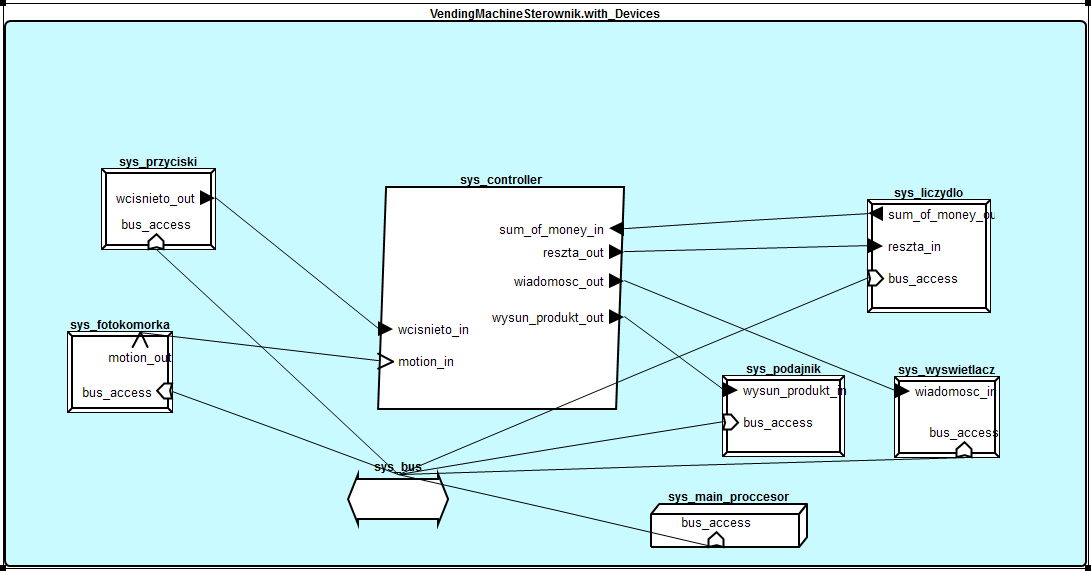
\includegraphics[scale=0.5]{./Diagrams/System}}
\caption{Diagram Systemu}
\end{figure}%
\begin{figure}[H]
\centerline{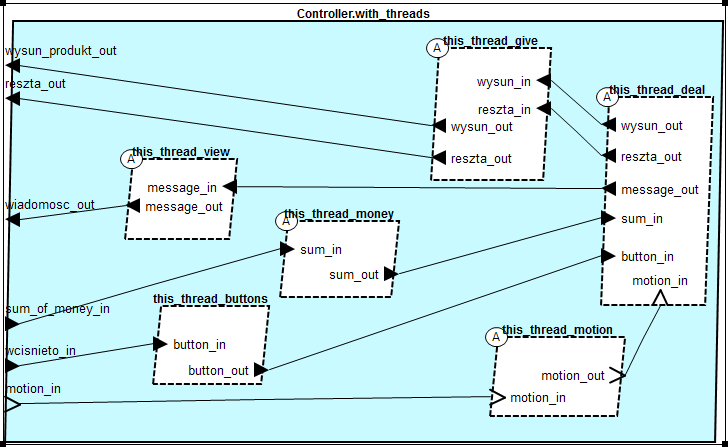
\includegraphics[scale=0.6]{./Diagrams/Controller}}
\caption{Diagram Kontrolera}
\end{figure}%

\begin{figure}[H]
\centerline{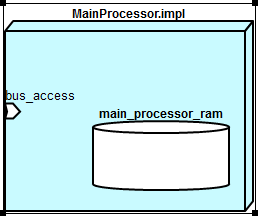
\includegraphics[scale=0.6]{./Diagrams/Procesor}}
\caption{Diagram Procesora}
\end{figure}%
\section{Uwagi}
Kod projekty w AADL'u i w C znajduje się w załącznikach.
%\bibliographystyle{unsrt}
%\bibliography{bib2}
\end{document}
